Hjertet består af to halvdele og er adskilt af en kraftig skillevæg. Ud over de to hjertehalvdele
består hjertet også af andre elementer, hér vigtigt at nævne hjerteklapperne, som sørger for,
at blodet kun kan løbe én vej. Hjertet har fire hjerteklapper: To AV-klapper, aortaklappen og
pulmonalklappen. Dette ses også på figur 1. Hjerteklappernes åbning og lukning bestemmes af trykket på henholdsvis den ene og den anden side. Højre side af hjertet pumper blod ud i lungekredsløbet via lungearterierne, også kaldt det lille kredsløb, mens venstre side af hjertet pumper blod ud i legemskredsløbet via aorta, også kaldt det store kredsløb. Hjertets pumpefunktionen er en vigtig funktion, der har til hovedopgave at transportere blod rundt i kroppen.

\begin{figure}[h!]
	\centering
	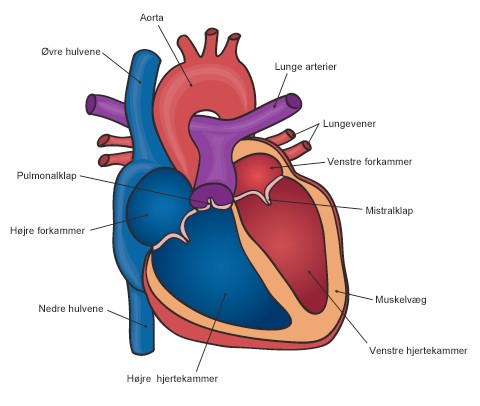
\includegraphics[width=0.5\linewidth]{Teori/Fysiologi/hjerte}
	\label{fig:hjerte}
	\caption{Figur af hjertets opbygning \cite{Hjerte}}
\end{figure}

For at hjertet kan transportere blodet rundt til hele kroppen kræver det et tryk, der dannes
ved, at hjertet trækker sig sammen med jævne mellemrum. Når hjertet slapper af, er blodtrykket
lavest - denne fase i hjertets cyklus kaldes diastolen, deraf kommer det diastoliske blodtryk. Når
hjertet i stedet kontraherer sig er blodtrykket højst - denne fase i hjertets cyklus kaldes systolen,
deraf kommer det systoliske blodtryk. 

\begin{figure}[h!]
	\centering
	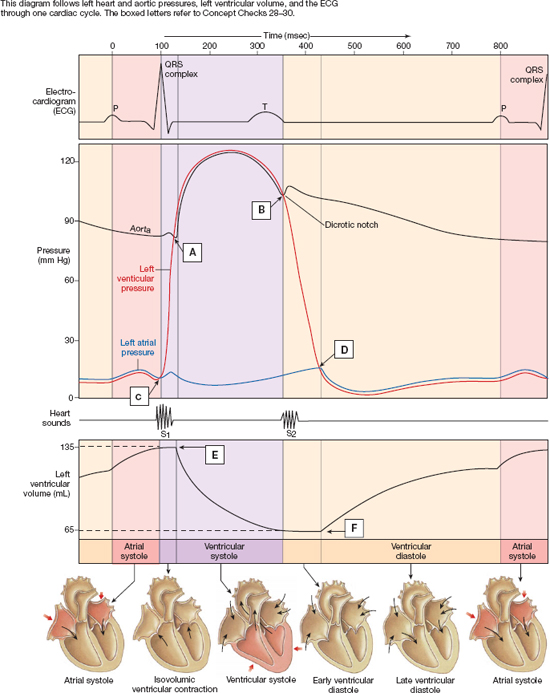
\includegraphics[width=0.7\linewidth]{Teori/Fysiologi/Blodtryk}
	\label{fig:blodtryk}
	\caption{Wiggers Diagram \cite{WiggersDiagram}}
\end{figure}

På figur 2 ved punkt c ses det, at systolen starter, når trykket i ventriklerne overstiger trykket i arterierne. AV-klapperne lukkes for at forhindre tilbagestrømning af blodet, der derved vil løbe i den forkerte retning. Når trykket i venstre ventrikel overstiger trykket i aorta åbnes aortaklappen og blodet vil strømme ud, dette ses ved punkt A. Ved punkt E ses det, at volumenet i ventriklerne falder idet blodet løber fra ventriklen til aorta, og videre ud i det store kredsløb som tidligere nævnt. 

På figur 2 ved punkt d ses det, at diastolen starter, når trykket i ventriklerne er lavere end i arterierne. Dette medfører, at den ene AV-klap åbnes, som det ses ved punkt b, så hjertet kan fyldes med blod. Under diastolen er aortaklappen lukket. Ved punkt F ses det, at volumenet i ventriklerne stiger, idet blodet løber fra atrierne til ventriklerne. 

Systolen starter, når trykket i ventriklerne igen overstiger trykket i arterierne. AV-klapperne
lukkes for at forhindre tilbagestrømning af blodet, der derved vil løbe i den forkerte retning. Når
trykket i venstre ventrikel overstiger trykket i aorta åbnes aortaklappen og blodet vil strømme
ud.

Blodtrykket måles som det tryk, der er højere end det atmosfæriske tryk. Det angives normalvis i mm Hg

Blodtryk kan måles invasivt eller non-invasivt. Da det er givet i problemformuleringen, at vi skal vise blodtrykket som funktion af tiden, vil dette projekt omhandle et invasivt blodtryksmålesystem. 
